% -*- latex -*-
%%%%%%%%%%%%%%%%%%%%%%%%%%%%%%%%%%%%%%%%%%%%%%%%%%%%%%%%%%%%%%%%
%%%%%%%%%%%%%%%%%%%%%%%%%%%%%%%%%%%%%%%%%%%%%%%%%%%%%%%%%%%%%%%%
%%%%
%%%% This text file is part of the lecture slides for
%%%% `Parallel Computing'
%%%% by Victor Eijkhout, copyright 2012-2021
%%%%
%%%% Subcomm-slides.tex : slides about communicator manipulation
%%%%
%%%%%%%%%%%%%%%%%%%%%%%%%%%%%%%%%%%%%%%%%%%%%%%%%%%%%%%%%%%%%%%%
%%%%%%%%%%%%%%%%%%%%%%%%%%%%%%%%%%%%%%%%%%%%%%%%%%%%%%%%%%%%%%%%

\begin{numberedframe}{Overview}
  In this section you will learn about various subcommunicators.

  Commands learned:
  \begin{itemize}
  \item \indexmpishow{MPI_Comm_dup}, discussion of library design
  \item \indexmpishow{MPI_Comm_split}
  \item discussion of groups
  \item discussion of inter/intra communicators.
  \end{itemize}
\end{numberedframe}

%\sectionframe{Motivation}

\begin{numberedframe}{Sub-computations}
  Simultaneous groups of processes, doing different tasks, but
  loosely interacting:
  \begin{itemize}
  \item Simulation pipeline: produce input data, run simulation, post-process.
  \item Climate model: separate groups for air, ocean, land, ice.
  \item Quicksort: split data in two, run quicksort independently on the halves.
  \item Process grid: do broadcast in each column.
  \end{itemize}
  New communicators are formed recursively from \indexmpishow{MPI_COMM_WORLD}.
\end{numberedframe}

\begin{numberedframe}{Communicator duplication}
Simplest new communicator: identical to a previous one.
\lstset{language=C++}
\begin{lstlisting}
int MPI_Comm_dup(MPI_Comm comm, MPI_Comm *newcomm)
\end{lstlisting}
This is useful for library writers:
\begin{lstlisting}
MPI_Isend(...); MPI_Irecv(...);
// library call
MPI_Waitall(...);  
\end{lstlisting}
\begin{itemize}
\item Naively, the library can `catch' the user messages.
\item With a duplicate communicator there is no confusion:\\
  user and library both have their own `context' for their messages.
\end{itemize}
\end{numberedframe}

\begin{numberedframe}{Interleaved library and user code}
  \cxxverbatimsnippet{catchmain}
\end{numberedframe}
\begin{numberedframe}{Library internally has messages}
  \cxxverbatimsnippet{catchcalls}
\end{numberedframe}
\begin{numberedframe}{Wrong way of setting up the library}
  \cxxverbatimsnippet{wrongcatchlib}
\end{numberedframe}

\begin{numberedframe}{Right way of setting up the library}
  \cxxverbatimsnippet{rightcatchlib}
\end{numberedframe}

\begin{numberedframe}{Disjoint splitting}
  Split a communicator in multiple disjoint others.
  
Give each process a `color', group processes by color:
\lstset{language=C}
\begin{lstlisting}
int MPI_Comm_split(MPI_Comm comm, int color, int key, 
                   MPI_Comm *newcomm)  
\end{lstlisting}
(\n{key} determines ordering: use rank unless you want special effects)
\end{numberedframe}

\begin{numberedframe}{Row/column example}
  Simulate a processor grid\\
  create subcommunicator per column (or row):
\begin{lstlisting}
MPI_Comm_rank( MPI_COMM_WORLD, &procno );
proc_i = procno % proc_column_length;
proc_j = procno / proc_column_length;

MPI_Comm column_comm;
MPI_Comm_split( MPI_COMM_WORLD, proc_j, procno, &column_comm );

MPI_Bcast( data, ... column_comm );
\end{lstlisting}
Food for thought: there are many columns,
but only one \n{column_comm} variable. Why?
\end{numberedframe}

\begin{numberedframe}{Row and column communicators}
  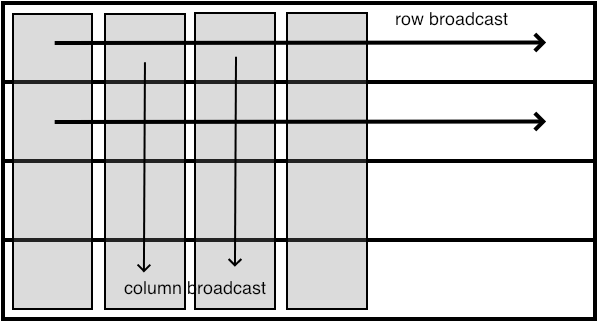
\includegraphics[scale=.4]{procgrid-bcast}

  Row and column broadcasts in subcommunicators
\end{numberedframe}

\begin{exerciseframe}[procgrid]
  \footnotesize
  \input ex:rowcolcomm
\end{exerciseframe}

\begin{exerciseframe}
  \input ex:recursivetranspose
\end{exerciseframe}

\begin{numberedframe}{Splitting by shared memory}
  \begin{itemize}
  \item
    \indexmpishow{MPI_Comm_split_type} splits into communicators of same type.
  \item Only supported type: \indexmpishow{MPI_COMM_TYPE_SHARED} splitting by
    shared memory.
  \end{itemize}

  \cverbatimsnippet{commsplittype}
\end{numberedframe}

\begin{numberedframe}{Inter-communicators}
\label{sl:comm-inter}
  \begin{itemize}
  \item Communicators so far are of \indextermsubh{intra}{communicator} type.
  \item Bridge between two communicators: \indextermsubh{inter}{communicator}.
  \item Example: communicator with newly spawned processes
  \end{itemize}  
\end{numberedframe}

\begin{numberedframe}{In a picture}
  \label{sl:intercomm-picture}
  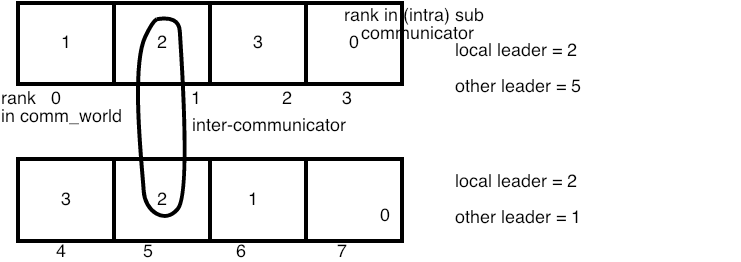
\includegraphics[scale=.4]{intercomm}

  Illustration of ranks in an inter-communicator setup
  \tiny\cverbatimsnippet{intercommcreate}
\end{numberedframe}

\begin{numberedframe}{Concepts}
  \label{sl:intercomm-concepts}
  \begin{itemize}
  \item Two local communicators
  \item The `peer' communicator that contains them
  \item Leaders in each of them
  \item An inter-communicator over the leaders.
  \end{itemize}
\end{numberedframe}

\begin{numberedframe}{Routines}
  \label{sl:intercomm-routines}
  \begin{itemize}
  \item
    \indexmpishow{MPI_Intercomm_create}: create
  \item \indexmpishow{MPI_Comm_get_parent}: the other leader (see process management)
  \item \indexmpishow{MPI_Comm_remote_size}, \indexmpishow{MPI_Comm_remote_group}:
    query the other communicator
  \item \indexmpishow{MPI_Comm_test_inter}: is this an inter or intra?
  \end{itemize}
\end{numberedframe}

\begin{numberedframe}{More}
  \begin{itemize}
  \item Non-disjoint subcommunicators through process groups.
  \item Process topologies: cartesian and graph.\\
    There will also be a section about this, later.
  \end{itemize}
\end{numberedframe}

\endinput

\begin{numberedframe}{}
\begin{lstlisting}
  
\end{lstlisting}
\end{numberedframe}

